%----------------------------------------------------------------------------------------
%	SOLUTION 5
%----------------------------------------------------------------------------------------
\subsection*{Problem 5}
\paragraph{(a)} The system dynamics given are as follows:
\begin{align}\label{eq:q5_ss_model}
	\alpha_k &= F \alpha_{k-1} + G u_{k-1} \nonumber\\
	y_k &= \tilde{y} + v_k = C\alpha_k + v_k,
\end{align}
where,
\begin{align*}
	F = \begin{bmatrix}-a_1 & 1\\-a_2 & 0\end{bmatrix},\ G = \begin{bmatrix}b_1\\b_2\end{bmatrix},\ C = \begin{bmatrix}1 & 0\end{bmatrix}.
\end{align*}
From~(\ref{eq:q5_ss_model}),
\begin{align}
	\tilde{y}_k &= C\alpha_k \nonumber\\
	&= C[F \alpha_{k-1} + G u_{k-1}] \nonumber\\
	&= CF \alpha_{k-1} + CG u_{k-1} \nonumber\\
	&= \begin{bmatrix}1 & 0\end{bmatrix}\begin{bmatrix}-a_1 & 1\\-a_2 & 0\end{bmatrix}\alpha_{k-1} + \begin{bmatrix}1 & 0\end{bmatrix}\begin{bmatrix}b_1\\b_2\end{bmatrix} u_{k-1} \nonumber\\
	&= \begin{bmatrix}-a_1 & 1\end{bmatrix}\alpha_{k-1} + b_1 u_{k-1} \nonumber\\
	&= -a_1\begin{bmatrix}1 & 0\end{bmatrix}\alpha_{k-1} + \begin{bmatrix}0 & 1\end{bmatrix}\alpha_{k-1} + b_1 u_{k-1} \nonumber\\
	&= -a_1 C \alpha_{k-1} + \begin{bmatrix}0 & 1\end{bmatrix}[F \alpha_{k-2} + G u_{k-2}] + b_1 u_{k-1} \nonumber\\
	&= -a_1 \tilde{y}_{k-1} + \begin{bmatrix}0 & 1\end{bmatrix}\begin{bmatrix}-a_1 & 1\\-a_2 & 0\end{bmatrix}\alpha_{k-2} + \begin{bmatrix}0 & 1\end{bmatrix}\begin{bmatrix}b_1\\b_2\end{bmatrix}u_{k-2} +b_1 u_{k-1}\nonumber\\
	&= -a_1\tilde{y}_{k-1} + \begin{bmatrix}-a_2 & 0\end{bmatrix}\alpha_{k-2} + b_2 u_{k-2} + b_1 u_{k-1} \nonumber\\
	&= -a_1 \tilde{y}_{k-1} - a_2 \tilde{y}_{k-2} + b_1 u_{k-1} + b_2 u_{k-2}.
\end{align}
Therefore, we can write it in the following matrix form
\begin{align}
	\tilde{y}_k = \underbrace{\begin{bmatrix}-\tilde{y}_{k-1} & -\tilde{y}_{k-2} & u_{k-1} & u_{k-2}\end{bmatrix}}_{H_k}\underbrace{\begin{bmatrix}a_1\\a_2\\b_1\\b_2\end{bmatrix}}_{x}.
\end{align}
Stacking all the $H_k$ for all $k \in \{2,3,\ldots,N\}$, we get
\begin{align*}
	\underbrace{\begin{bmatrix}\tilde{y}_2\\\tilde{y}_3\\\vdots\\\tilde{y}_N\end{bmatrix}}_{\tilde{y}} = \underbrace{\begin{bmatrix}-\tilde{y}_{1} & -\tilde{y}_0 & u_1 & u_0\\-\tilde{y}_2 & -\tilde{y}_1 & u_2 & u_1\\ \vdots & \vdots & \vdots & \vdots\\-\tilde{y}_{N-1} & -\tilde{y}_{N-2} & u_{N-1} & u_{N-2}\end{bmatrix}}_{H} \underbrace{\begin{bmatrix}a_1\\a_2\\b_1\\b_2\end{bmatrix}}_{x},
\end{align*}
where $N$ is the total number of measurements.
\paragraph{(b)} Using the ordinary least squares (OLS) method, we get the following estimate of $x$:
\begin{align}
	\hat{x}_{OLS} = \begin{bmatrix}0.5\\0.25\\1.0\\0\end{bmatrix}
\end{align}
I have also implemented recursive least squares (RLS) method and got the following estimate of $x$:
\begin{align}
\hat{x}_{RLS} = \begin{bmatrix}0.52\\0.27\\1.0\\0.02\end{bmatrix}.
\end{align}
\paragraph{(c), (d)}After adding the noise with $\sigma = 0.1$ and running the OLS and RLS methods I got the following estimates of state vector $x$:
\begin{align}
	\hat{x}_{OLS} = \begin{bmatrix}0.036\\-0.019\\0.927\\-0.383\end{bmatrix},\ \hat{x}_{RLS} = \begin{bmatrix}0.036\\-0.019\\0.927\\-0.383\end{bmatrix}.
\end{align}
\paragraph{(e)}After adding the noise with $\sigma = 0.001$ and running the OLS and RLS methods I got the following estimates of state vector $x$:
\begin{align}
\hat{x}_{OLS} = \begin{bmatrix}0.475\\0.234\\0.996\\-0.021\end{bmatrix},\ \hat{x}_{RLS} = \begin{bmatrix}0.476\\0.235\\0.996\\-0.020\end{bmatrix}.
\end{align}
Therefore, we can see that the system is very sensitive to noise. Reducing the noise variance greatly improved the estimates to produce values closer to the estimate calculated in part (b) with $0$ noise.
\paragraph{(f)} To validate the accuracy of the estimates we can run cross-validation where we choose $N_{train} < N$ number of time index randomly from the available data and construct the $H_{train} \in \mathbb{R}^{N_{train}\times 4}$ matrix based on those time index and then use OLS / RLS to estimate $\hat{x}_{train}$ based on those randomly chosen time index. Then we can use the rest $N_{val} = N-N_{train}$ number of points from the available data and construct the $H_{val} \in \mathbb{R}^{N_{val}\times 4}$ and then predict $y_{val} \in \mathbb{R}^{N_{val}}$ based on $H_{val}$ and $\hat{x}_{train}$. Now we can compute the root mean square error from $y_{val}$ and $y$ values from the original dataset. We can perform the operation for many times choosing different time index for train and test and then take the mean and standard deviation to show the confidence of the estimates.

I have used $10$-fold cross validation for this purpose. Fig.~\ref{fig:q5_val_error} shows the validation error plot for three different noise standard deviation, $0.1, 0.01, 0.001$. The line connect the mean values of the root mean square error collected for each fold for each noise variance. $x$-axis denotes the noise standard deviation.
\begin{figure}[h]
	\centering
	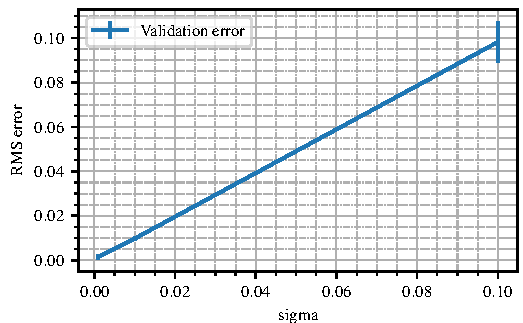
\includegraphics[scale=1.0,trim={0cm 0cm 0cm 0cm},clip]{./code/generatedPlots/val_error.pdf}
	\label{fig:q5_val_error}
	\caption{Q5.f: Validation error plot for $\sigma=0.1, 0.01, 0.001$}
\end{figure}
Thus we can see that the root mean square error increases with increase in noise variance which indicates lower confidence in the estimates of $x$. Table~\ref{tbl:5_f_folds} shows the RMS error for each folds of the cross validation and Table~\ref{tbl:5_f_mean_std} shows the mean and standard deviation across all the folds for each noise standard deviation.
\begin{table}[ht]
	\centering
	\caption{Q5.f: Error table for 10-fold cross validation}
	\begin{tabular}[t]{ccccccccccc} 
		\hline
		& fold $1$ & fold $2$ & fold $3$ & fold $4$ & fold $5$ & fold $6$ & fold $7$ & fold $8$ & fold $9$ & fold $10$\\ [0.5ex] 
		\hline
		$\sigma_{noise}=0.001$ & $0.005$ & $0.001$ & $0.001$ & $0.001$ & $0.001$ & $0.001$ & $0.001$ & $0.001$ & $0.001$ & $0.001$\\
		$\sigma_{noise}=0.01$ & $0.012$ & $0.009$ & $0.011$ & $0.009$ & $0.01$ & $0.01$ & $0.008$ & $0.011$ & $0.008$ & $0.009$\\
		$\sigma_{noise}=0.1$ & $0.09$ & $0.09$ & $0.11$ & $0.10$ & $0.09$ & $0.10$ & $0.08$ & $0.11$ & $0.11$ & $0.10$\\[1ex]
		\hline
	\end{tabular}
	\label{tbl:5_f_folds}
\end{table}
\begin{table}[ht]
	\centering
	\caption{Q5.f: Mean and Std of RMS error}
	\begin{tabular}[t]{ccc} 
		\hline
		$\sigma_{noise}$ & Mean & Standard deviation\\ [0.5ex] 
		\hline
		$0.001$ & $0.001$ & $0.001$\\
		$0.01$ & $0.01$ & $0.001$\\
		$0.1$ & $0.098$ & $0.009$\\[1ex]
		\hline
	\end{tabular}
	\label{tbl:5_f_mean_std}
\end{table}
\paragraph{Git location of the code:} The code file has been attached as a PDF file. Moreover, the code can be found at\\
\url{https://github.umn.edu/dey00011/EE5251\_optimal\_filter\_estimation/tree/master/HW2/code}
